\section{Multicast}

How to efficiently transmit data to a set of receivers. One or many to many.

\paragraph{Source-Based}
Sender simply sends as many copies of each IP packet as there are receivers (replication). Easy to implement but wastes a lot of bandwidth and is therefore not efficient.

\paragraph{Network-Based}
Sender transmit one copy of each IP packet like in IP unicast and network (i.e. the routers) take care of distributing this information to all the receivers (distribution tree). Efficient since each packet crosses each link only once but hard to implement (needs new protocols and forwarding mechanisms). Group of receivers is identified by a group address (multicast IP address).

\subsection{IP Multicast}

%TODO IPTV, IGMP and PIM, MOSPF

\paragraph{Addressing A Group Of Receivers}
A subset of the IP address space is reserved for multicast, namely 224.0.0.0 - 239.255.255.255 (leading bits are 1110) with some having pre-defined allocations (all hosts, all OSPF routers, etc.). Some of these can only be used within an AS (no public routing), namely 239.0.0.0 - 239.255.255.255.

\paragraph{Receiving Multicast Traffic}
On top of the physical MAC (L2) address (start with 0 in first byte), we can tell a host to listen to additional ones (logical addresses that identify a group of Ethernet destinations and start with 1 in first byte).

\paragraph{Multicast Address to MAC Mapping}
Take the 32-bit IPv4 multicast address and trim away the first 8 bits. The remaining 23 bits are the last 23 bits of the corresponding MAC address that always start with the same 25 bits (01:00:5e).

This process is not lossless, meaning that 32 IP multicast addresses are always mapped to the same logical Ethernet address. This can lead to unwanted traffic. Host needs to check the IP address and discard unwanted packets.

\paragraph{Router: Which Host is in Which Group?}
The Internet Group Management Protocol (IGMP) is used by hosts and adjacent routers (first-hop) to create multicast group membership. Hosts (repeatedly) tell / request from routers that they want the traffic with a specific IP destination address and routers keep track of that. Routers also periodically send out subscription queries. Adjacent routers use Protocol Independent Multicast (PIM) to direct traffic from hosts sending multicast traffic to hosts that requested it.

\paragraph{Dynamic Construction of Distribution Trees}
How do routers learn where the various receivers are and keep track of those over time (and where are the sources)?

\textbf{Pro-Active:} Hosts use IGMP to establish subscriptions and tell their first-hop routers and then a routing protocol is used to distribute group memberships s.t. each router knows the exact location of each group member (e.g. extend a link-state protocol as in MOSPF). Each router computes the shortest path tree (S, G) for each source S (original senders of multicast traffic) and group G (on demand whenever router receives a packet for G). Routers have full knowledge but memory overhead for all routers, flooding competes with normal link-state messages and as the number of sources and groups grows, computing the SPT can become problematic.

\textbf{Reactive:} Routers assume that receivers are everywhere and will initially broadcast the traffic (along shortest path tree with source as root) - only flood traffic when it arrives from SP upstream (Reverse Path Filtering - RPF). Unwanted branches are pruned by receiving stop requests from downstream routers that are not interested (or edge routers indicating that they have no hosts interested in traffic). This is called Flood-and-Prune. Approach is simple (plug and play) but costly since routers need to maintain per (S, G) state and flooding is frequently reactivated. There is also the hybrid mode that uses rendez-vous points: one router is the root of a shared distribution tree per group (configured in advance) and all routers know the address  - sources then encapsulate traffic to root and it multicasts the decapsulated traffic alongside shared traffic. Receivers dynamically join the shared tree.

\begin{figure}[h]
	\centering
	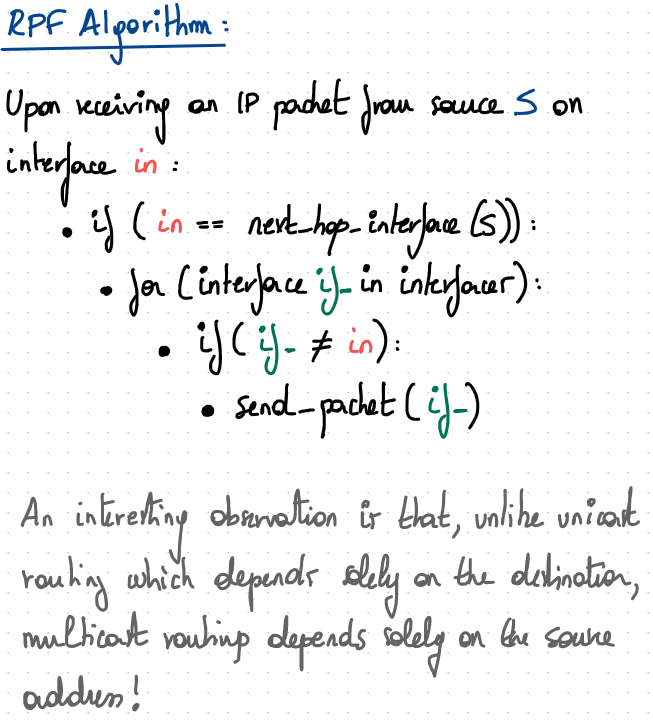
\includegraphics[scale=0.6]{images/5-rpf.PNG}
	\caption{Algo for Reverse Path Filtering.}
	\label{fig:rpf}
\end{figure}

\textbf{Avoiding Unnecessary Transmissions:} Sender-based solutions include each router computing the list of interfaces for each possible source on which to broadcast to s.t. it only includes interfaces on the SPT from a source (routers can rely on learned network topology). Receiver-based solutions include each router learning the list of outgoing interfaces on which to broadcast from for each source by having downstream routers tell them that a given interface is not on the shortest path (less intensive than sender-based) - router just broadcasts and downstream sends stop messages (as described in the Flood-and-Prune method).

%TODO ??

\textbf{Protocol Independent Multicast:} Most widely deployed multicast routing protocol. It leverages the existing unicast routing table to perform receiver-based optimization for RPF. Two modes: dense (Flood-and-Prune) or sparse (Rendez-Vous Points).

%TODO look this up
